\documentclass[DaoFP]{subfiles}
\begin{document}
\setcounter{chapter}{1}
\chapter{组合}

\section{组合}

编程的核心在于组合。借用维特根斯坦的话,可以说:"对于不可分解之物,我们应当保持沉默。"这不是禁令,而是事实陈述。研究、理解和描述的过程就是分解的过程;我们的语言也反映了这一点。

我们构建对象和箭头的词汇表,正是为了表达组合的思想。

给定一个从$a$到$b$的箭头$f$和一个从$b$到$c$的箭头$g$,它们的组合是一个直接从$a$到$c$的箭头。换句话说,如果有两个箭头,其中一个的目标与另一个的源相同,我们总是可以将它们组合得到第三个箭头。

\[
 \begin{tikzcd}
 a
 \arrow[rr, bend left, "h"]
 \arrow[r, "f"']
 & b
 \arrow[r, "g"']
& c
 \end{tikzcd}
\]

在数学中,我们用一个小圆圈表示组合
\[h = g \circ f\]
我们这样读:"$h$等于$f$之后的$g$"。选择"之后"这个词暗示了动作的时间顺序,在大多数情况下这是一个有用的直觉。

组合的顺序可能看起来是反的,但这是因为我们认为函数是从右边接受参数的。
在Haskell中,我们用点代替圆圈:
\begin{haskell}
h = g . f
\end{haskell}
这就是每个程序的精髓。为了实现\hask{h},我们将其分解为更简单的问题\hask{f}和\hask{g}。这些又可以进一步分解,依此类推。

现在假设我们能够将$g$本身分解为$j \circ k$。我们有
\[h = (j \circ k) \circ f\]
我们希望这个分解与
\[h = j \circ (k \circ f)\]
相同。我们希望能够说我们将$h$分解为三个更简单的问题
\[h =  j \circ k \circ f\]
而不必跟踪哪个分解先进行。这被称为组合的\emph{结合性},从现在起我们将假设这一点。

组合产生了两种箭头映射,称为前组合和后组合。

当你\index{后组合}\emph{后组合}一个箭头$h$与一个箭头$f$时,它产生箭头$f \circ h$(箭头$f$在箭头$h$之后应用)。当然,你只能将$h$与源为$h$的目标的箭头进行后组合。通过$f$的后组合写为$(f \circ -)$,为$h$留一个空位。正如老子所说:"后组合的用处来自于不存在的东西。"

因此,一个箭头$f \colon a \to b$诱导了一个箭头映射$(f \circ -)$,它将探测$a$的箭头映射到探测$b$的箭头。

\[
 \begin{tikzcd}
 \node (a1) at (0, 2) {};
 \node (a2) at (-0.5, 2) {};
 \node (a3) at (0.5, 2) {};
 \node (aa) at (0.5, 1) {};
 \node(a) at (0, 0) {a};
 \draw[->, red] (a1) -- (a);
 \draw[->] (a2) -- (a);
 \draw[->, blue] (a3) -- (a);
 \node (b1) at (3+0, 2) {};
 \node (b2) at (3-0.5, 2) {};
 \node (b3) at (3+0.5, 2) {};
 \node (bb) at (2.5, 1) {};
 \node(b) at (3, 0) {b};
 \draw[->, red] (b1) -- (b);
 \draw[->] (b2) -- (b);
 \draw[->, blue] (b3) -- (b);
 \draw[->] (a) -- node[below]{f} (b);
 \draw[->, dashed] (aa) -- node[above]{(f \circ -)} (bb);
  \end{tikzcd}
\]
由于对象没有\emph{内部}结构,当我们说$f$将$a$转换为$b$时,这正是我们的意思。

后组合让我们能够将焦点从一个对象转移到另一个对象。

对偶地,你可以\index{前组合}\emph{前组合}通过$f$,或者应用$(- \circ f)$将源自$b$的箭头映射到源自$a$的箭头(注意方向的变化)。

\[
 \begin{tikzcd}
 \node (a1) at (0, -2) {};
 \node (a2) at (-0.5, -2) {};
 \node (a3) at (0.5, -2) {};
 \node (aa) at (0.5, -1) {};
 \node(a) at (0, 0) {a};
 \draw[<-, red] (a1) -- (a);
 \draw[<-] (a2) -- (a);
 \draw[<-, blue] (a3) -- (a);
 \node (b1) at (3+0, -2) {};
 \node (b2) at (3-0.5, -2) {};
 \node (b3) at (3+0.5, -2) {};
 \node (bb) at (2.5, -1) {};
 \node(b) at (3, 0) {b};
 \draw[<-, red] (b1) -- (b);
 \draw[<-] (b2) -- (b);
 \draw[<-, blue] (b3) -- (b);
 \draw[->] (a) -- node[above]{f} (b);
 \draw[->, dashed] (bb) -- node[below]{(- \circ f)} (aa);
  \end{tikzcd}
\]

前组合让我们能够将视角从观察者$b$转移到观察者$a$。

前组合和后组合是箭头的映射。由于箭头形成集合,这些是集合之间的\emph{函数}。

另一种看待前组合和后组合的方式是,它们是双孔组合运算符$(- \circ -)$的部分应用的结果,我们可以在其中一个孔中预先填充一个固定的箭头。

在编程中,一个出向箭头被解释为从其源中提取数据。一个入向箭头被解释为生成或构造目标。出向箭头定义了接口,入向箭头定义了构造函数。

对于Haskell程序员,这里是将后组合实现为高阶函数的方式:
\begin{haskell}
postCompWith :: (a -> b) -> (x -> a) -> (x -> b)
postCompWith f = \h -> f . h
\end{haskell}
类似地,前组合的实现如下:
\begin{haskell}
preCompWith :: (a -> b) -> (b -> x) -> (a -> x)
preCompWith f = \h -> h . f
\end{haskell}

做以下练习,以使自己相信焦点和视角的转移是可组合的。
\begin{exercise}\label{ex-yoneda-composition}
假设你有两个箭头,$f \colon a \to b$和$g \colon b \to c$。它们的组合$g \circ f$诱导了一个箭头映射$((g \circ f) \circ -)$。证明如果你先应用$(f \circ -)$,然后再应用$(g \circ -)$,结果是一样的。符号上:
\[((g \circ f) \circ -) = (g \circ -) \circ (f \circ -)\]

提示:选择一个任意对象$x$和一个箭头$h \colon x \to a$,看看你是否得到相同的结果。注意,这里的$\circ$是重载的。在右边,当放在两个后组合之间时,它表示常规的函数组合。
\end{exercise}

\begin{exercise}
使自己相信前一个练习中的组合是结合的。提示:从三个可组合的箭头开始。
\end{exercise}

\begin{exercise}
证明前组合$(- \circ f)$是可组合的,但组合的顺序是相反的:
\[(- \circ (g \circ f)) = (- \circ f) \circ (- \circ g) \]
\end{exercise}
\section{函数应用}

我们已经准备好编写第一个程序了。有句俗话说:"千里之行,始于足下。"考虑从$1$到$b$的旅程。我们的第一步可以是从终端对象$1$到某个$a$的箭头。它是$a$的一个元素。我们可以将其写为:
\[1 \xrightarrow x a \]
旅程的其余部分是箭头:
\[a \xrightarrow f b\]
这两个箭头是可组合的(它们在中间共享对象$a$),它们的组合是从$1$到$b$的箭头$y$。换句话说,$y$是$b$的一个\emph{元素}:

\[
 \begin{tikzcd}
 1
 \arrow[rr, bend left, "y"]
 \arrow[r, "x"']
 & a
 \arrow[r, "f"']
& b
 \end{tikzcd}
\]
我们可以将其写为:
\[y = f \circ x \]

我们使用$f$将$a$的一个\emph{元素}映射到$b$的一个\emph{元素}。由于这是我们经常做的事情,我们称之为函数$f$对$x$的\emph{应用},并使用简写符号
\[y = f x \]
让我们将其翻译成Haskell。我们从$a$的一个元素$x$开始(\hask{x :: ()-> a}的简写)
\begin{haskell}
x :: a
\end{haskell}
我们将函数$f$声明为从$a$到$b$的"箭头对象"的一个元素
\begin{haskell}
f :: a -> b
\end{haskell}
并理解(稍后将详细说明)它对应于从\hask{a}到\hask{b}的箭头。结果是$b$的一个元素
\begin{haskell}
y :: b
\end{haskell}
并且它被定义为
\begin{haskell}
y = f x
\end{haskell}
我们称之为函数对参数的应用,但我们能够纯粹用函数组合来表达它。(注意:在其他编程语言中,函数应用需要使用括号,例如\hask{y = f(x)}。)
\section{恒等态射}

你可以将箭头视为表示变化:对象 $a$ 变为对象 $b$。一个回环的箭头表示对象自身的变化。但变化有其对偶面:不变、无为,或者如老子所说的 \emph{无为}。

每个对象都有一个特殊的箭头,称为恒等态射(identity),它使对象保持不变。这意味着,当你将这个箭头与任何其他箭头(无论是进入的还是离开的)进行复合时,你得到的仍然是那个箭头。从动作的角度来看,恒等态射什么都不做,也不花费时间。

对象 $a$ 上的恒等态射称为 $id_a$。因此,如果我们有一个箭头 $f \colon a \to b$,我们可以将其与两边的恒等态射进行复合:

\[id_b \circ f = f = f \circ id_a \]
或者,用图示表示为:
\[
 \begin{tikzcd}
 a
 \arrow[loop, "id_a"']
 \arrow[r, "f"]
 & b
 \arrow[loop, "id_b"']
 \end{tikzcd}
\]

我们可以很容易地检查恒等态射对元素的作用。取一个元素 $x \colon 1 \to a$ 并将其与 $id_a$ 复合。结果是:
\[id_a \circ x = x\]
这意味着恒等态射使元素保持不变。

在 Haskell 中,我们对所有恒等函数使用相同的名称 \hask{id}(我们不会在其上加上它所作用的类型的下标)。上述方程,指定了 $id$ 对元素的作用,直接翻译为:
\begin{haskell}
id x = x
\end{haskell}
这成为函数 \hask{id} 的定义。

我们之前看到,初始对象和终止对象都有唯一的箭头回环到它们自身。现在我们说,每个对象都有一个恒等态射回环到它自身。记住我们关于唯一性的说法:如果你能找到两个这样的箭头,那么它们必须相等。我们必须得出结论,我们之前讨论的这些唯一的回环箭头必须是恒等态射。我们现在可以标记这些图示:

\[
 \begin{tikzcd}
 \hask{Void}
 \arrow[loop, "id"']
 \end{tikzcd}
 \begin{tikzcd}
 \hask{()}
 \arrow[loop, "id"']
 \end{tikzcd}
\]

在逻辑中,恒等态射翻译为重言式。这是一个平凡的证明,即“如果 $a$ 为真,那么 $a$ 为真”。它也被称为 \emph{同一性规则}。

如果恒等态射什么都不做,那么我们为什么还要关心它?想象一下,你去旅行,复合了几个箭头,然后发现自己回到了起点。问题是:你做了什么,还是你浪费了时间?回答这个问题的唯一方法是将你的路径与恒等态射进行比较。

有些往返带来了变化,而有些则没有。

更重要的是,恒等态射将允许我们比较对象。它们是同构定义的一个组成部分。

\begin{exercise}\label{ex-yoneda-identity}
$(id_a \circ -)$ 对终止于 $a$ 的箭头做了什么?$(- \circ id_a)$ 对从 $a$ 出发的箭头做了什么?
\end{exercise}
\section{单态射}

考虑函数 \hask{even},它测试输入是否能被2整除:
\begin{haskell}
even :: Int -> Bool
\end{haskell}
这是一个多对一的函数:所有偶数都被映射到 \hask{True},所有奇数都被映射到 \hask{False}。关于输入的大部分信息都被丢弃了,我们只关心它的奇偶性,而不是它的实际值。通过丢弃信息,我们得到了一个抽象\footnote{抽象的字面意思是提取}。函数(以及后来的函子)是抽象的典型代表。

与此形成对比的是函数 \hask{injectBool}:
\begin{haskell}
injectBool :: Bool -> Int
injectBool b = if b then 1 else 0
\end{haskell}
这个函数不会丢弃信息。你可以从它的结果中恢复它的参数。

不丢弃信息的函数也很有用:它们可以被视为将其源注入到目标中。你可以将源的类型想象为一个被嵌入到目标中的\emph{形状}。在这里,我们将一个两元素的形状 \hask{Bool} 嵌入到整数类型中。

\[
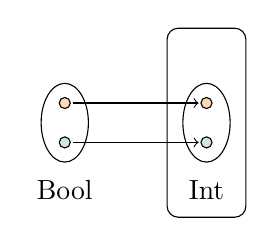
\begin{tikzpicture}
   \def\Xa{0};
   \def\Xb{1.8}       
   \def\Y{0};
   \def\Yb{-0.85};
   \def\delta{0.1};
  
         \draw(\Xa, \Y) ellipse (0.3 and 0.5);
	% dots
        \draw (\Xa, \Y + 0.25) [fill=orange!30] circle (2pt);
        \draw (\Xa, \Y - 0.25) [fill=blue!50!green!20] circle (2pt);
        
        \draw [rounded corners] (\Xb - 0.5, \Y - 1.2) rectangle (\Xb + 0.5, \Y + 1.2) {};
        \draw(\Xb, \Y) ellipse (0.3 and 0.5);
	% dots
        \draw (\Xb, \Y + 0.25) [fill=orange!30] circle (2pt);
        \draw (\Xb, \Y - 0.25) [fill=blue!50!green!20] circle (2pt);
        % arrows
        \draw [->] (\Xa + \delta, \Y - 0.25) -- (\Xb - \delta, \Y - 0.25);
        \draw [->] (\Xa + \delta, \Y + 0.25) -- (\Xb - \delta, \Y + 0.25);
        % labels
        \node at (\Xa, \Yb) {Bool};
        \node at (\Xb, \Yb) {Int};
\end{tikzpicture}
\]

单射函数,或\index{单射}\emph{单射},被定义为总是将不同的值分配给不同的参数。换句话说,它们不会将多个元素合并为一个。

这是另一种稍微复杂的说法:单射将两个元素映射到一个元素,仅当这两个元素相等时。

我们可以通过将“元素”替换为从终端对象出发的箭头,将这个定义翻译为范畴论语言。我们会说,$f \colon a \to b$ 是一个单射,如果对于任何一对全局元素 $x_1 \colon 1 \to a$ 和 $x_2 \colon 1 \to a$,以下蕴含成立:
\[ f \circ x_1 = f \circ x_2 \implies x_1 = x_2 \]

\[
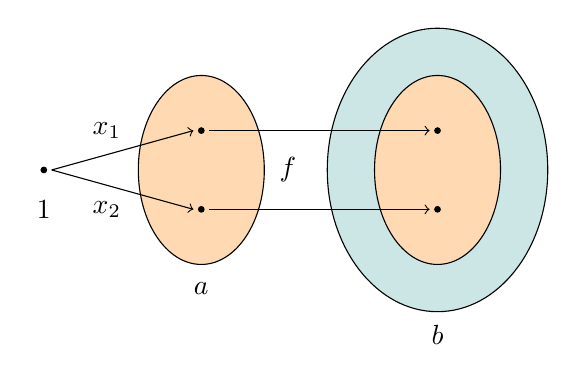
\begin{tikzpicture}
  \def\X{-2.0}
  \def\Xa{0};
  \def\Xmid{1.1};
  \def\Xb{3};
  \def\delta{0.1};
  
  \def\Ymid{0};
  \def\Ytip{-0.9};
  \def\Ybot{-1.5};
         \draw (\Xa , \Ymid)[fill=orange!30]  ellipse (0.8 and 1.2);
         \draw (\Xb, \Ymid)[fill=blue!50!green!20]   ellipse (1.4 and 1.8);
         \draw (\Xb , \Ymid) [fill=orange!30]  ellipse (0.8 and 1.2);
	% dots
        \filldraw (\X, \Ymid) circle (1pt);
        \filldraw (\Xa, \Ymid - 0.5) circle (1pt);
        \filldraw (\Xa, \Ymid + 0.5) circle (1pt);
        \filldraw (\Xb, \Ymid - 0.5) circle (1pt);
        \filldraw (\Xb, \Ymid + 0.5) circle (1pt);

	% arrows 
	\draw [->] (\X + \delta, \Ymid) --  (\Xa - \delta, \Ymid + 0.5);
	\draw [->] (\X + \delta, \Ymid)  -- (\Xa - \delta, \Ymid - 0.5);
	\draw [->] (\Xa + \delta, \Ymid + 0.5) --  (\Xb - \delta, \Ymid + 0.5);
	\draw [->] (\Xa + \delta, \Ymid - 0.5)  -- (\Xb - \delta, \Ymid - 0.5);
	
	% labels
	\node at (\Xmid, \Ymid) { $f$ };
	\node at (\X + 0.8, \Ymid + 0.5) { $x_1$ };
	\node at (\X + 0.8, \Ymid - 0.5) { $x_2$ };
	\node at (\X, \Ymid - 0.5) {$1$};
	\node at (\Xa, \Ybot) {$a$};
	\node at (\Xb, \Ybot - 0.6) {$b$};

\end{tikzpicture}
\]

这个定义的问题在于,并非每个范畴都有终端对象。一个更好的定义是用任意形状替换全局元素。因此,单射性的概念被推广为单态射。

一个箭头 $f \colon a \to b$ 是\index{单态射}\emph{单态射},如果对于任何对象 $c$ 和一对箭头 $g_1 \colon c \to a$ 和 $g_2 \colon c \to a$,我们有以下蕴含:
\[ f \circ g_1 = f \circ g_2 \implies g_1 = g_2 \]

要证明一个箭头 $f \colon a \to b$ \emph{不是}单态射,只需找到一个反例:$a$ 中的两个不同形状,使得 $f$ 将它们映射到 $b$ 中的相同形状。

单态射,或简称“monos”,通常用特殊箭头表示,如 $a \hookrightarrow b$ 或 $a \rightarrowtail b$。

在范畴论中,对象是不可分割的,因此我们只能通过箭头来讨论子对象。我们说单态射 $a \hookrightarrow b$ 选择了 $b$ 的一个子对象,其形状为 $a$。

\begin{exercise}
证明从终端对象出发的任何箭头都是单态射。
\end{exercise}
\section{满同态}

函数 \hask{injectBool} 是单射的(因此是一个单同态),但它只覆盖了目标集合的一小部分——在无限多个整数中仅覆盖了两个。
\begin{haskell}
injectBool :: Bool -> Int
injectBool b = if b then 1 else 0
\end{haskell}
相比之下,函数 \hask{even} 覆盖了整个 \hask{Bool}(它可以生成 \hask{True} 和 \hask{False})。覆盖整个目标集合的函数被称为\index{满射}\emph{满射}。

为了推广单射,我们使用了额外的“映射入”。为了推广满射,我们将使用“映射出”。满射在范畴论中的对应物被称为满同态。

一个箭头 $f \colon a \to b$ 是一个\index{满同态}\emph{满同态},如果对于任意对象 $c$ 和一对箭头 $g_1 \colon b \to c$ 和 $g_2 \colon b \to c$,我们有以下蕴含关系:
\[ g_1 \circ f = g_2 \circ f \implies g_1 = g_2 \]
反之,要证明 $f$ 不是满同态,只需选择一个对象 $c$ 和两个不同的箭头 $g_1$ 和 $g_2$,它们在 $f$ 的复合下一致。

为了理解这个定义,我们需要可视化“映射出”。正如“映射入”一个对象可以被视为定义形状一样,“映射出”一个对象可以被视为定义该对象的属性。

在处理集合时,这一点尤为明显,特别是当目标集合是有限的。你可以将目标集合的元素视为定义一种颜色。所有映射到该元素的源集合元素都被“涂上”特定的颜色。例如,函数 \hask{even} 将所有偶数整数涂上 \hask{True} 颜色,将所有奇数整数涂上 \hask{False} 颜色。

在满同态的定义中,我们有两个这样的映射,$g_1$ 和 $g_2$。假设它们只有微小的差异。对象 $b$ 的大部分区域被它们涂成相同的颜色。

\[
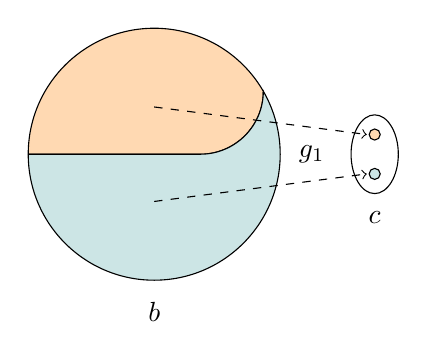
\begin{tikzpicture}
  \def\Xa{0};
  \def\Xmid{1.2};
  \def\Xb{3.2};
  \def\Xc{6};
  \def\delta{0.1};
  \def\d{0.3};
  \def\R{0.8};
  
  \def\Y{0};
  \def\Ybot{-2};
  
         \draw(\Xc, \Y) ellipse (0.3 and 0.5);
         % areas
        \draw [fill=orange!30] (\Xb - 2 * \R, \Y) 
        arc[start angle=180, delta angle=-180+30, radius=2 * \R]
        arc[start angle=0, delta angle=-90, radius=\R]
         to (\Xb - 2 * \R, \Y);
         
         \draw [fill=blue!50!green!20]  (\Xb - 2 * \R, \Y)
         arc[start angle=-180, delta angle=180+30, radius=2 * \R]
         arc[start angle=0, end angle=-90, radius=\R] 
         to (\Xb - 2 * \R, \Y);

	% dots
        \draw (\Xc, \Y + 0.25) [fill=orange!30] circle (2pt);
        \draw (\Xc, \Y - 0.25) [fill=blue!50!green!20] circle (2pt);

	% arrows
	\draw[->, dashed] (\Xb, \Y + 0.6) -- (\Xc - \delta, \Y + 0.25);
	\draw[->, dashed] (\Xb, \Y - 0.6) -- (\Xc - \delta, \Y - 0.25);
	% labels
	\node at (\Xc - 0.8, \Y) { $g_1$ };
	\node at (\Xb, \Ybot) {$b$};
	\node at (\Xc, \Y - 0.8) {$c$};
\end{tikzpicture}
\hspace{1cm}
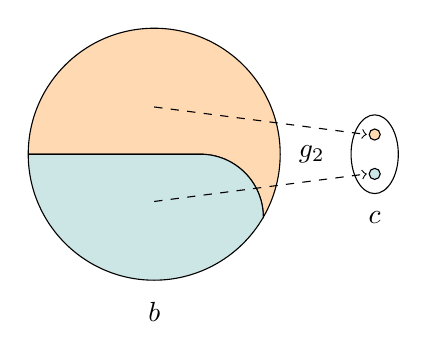
\begin{tikzpicture}

  \def\Xa{0};
  \def\Xmid{1.2};
  \def\Xb{3.2};
  \def\Xc{6};
  \def\delta{0.1};
  \def\d{0};
  \def\R{0.8};
  
  \def\Y{0};
  \def\Ybot{-2};
  
         \draw(\Xc, \Y) ellipse (0.3 and 0.5);
         % areas
          \draw [fill=orange!30] (\d + \Xb - 2 * \R, \Y) 
         arc[start angle=180, delta angle=-180-30, radius=2 * \R]
         arc[start angle=0, delta angle=90, radius=\R]
         to (\d + \Xb - 2 * \R, \Y);
         
         \draw [fill=blue!50!green!20]  (\d + \Xb - 2 * \R, \Y)
         arc[start angle=-180, delta angle=180-30, radius=2 * \R]
         arc[start angle=0, end angle=90, radius=\R] 
         to (\d + \Xb - 2 * \R, \Y);
         
	% dots
        \draw (\Xc, \Y + 0.25) [fill=orange!30] circle (2pt);
        \draw (\Xc, \Y - 0.25) [fill=blue!50!green!20] circle (2pt);
        
	% arrows
	\draw[->, dashed] (\Xb, \Y + 0.6) -- (\Xc - \delta, \Y + 0.25);
	\draw[->, dashed] (\Xb, \Y - 0.6) -- (\Xc - \delta, \Y - 0.25);
	% labels
	\node at (\Xc - 0.8, \Y) { $g_2$ };
	\node at (\Xb, \Ybot) {$b$};
	\node at (\Xc, \Y - 0.8) {$c$};
\end{tikzpicture}
\]

如果 $f$ \emph{不是}满同态,那么它的像可能只覆盖了 $g_1$ 和 $g_2$ 涂色相同的部分。这两个箭头在 $f$ 的复合下对 $a$ 的涂色一致,尽管它们在整体上是不同的。

\[
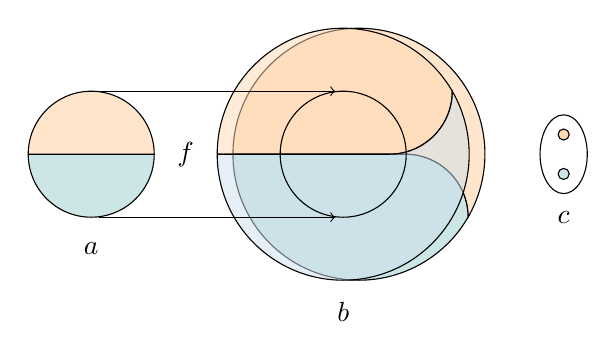
\begin{tikzpicture}
  \def\Xa{0};
  \def\Xmid{1.2};
  \def\Xb{3.2};
  \def\Xc{6};
  \def\delta{0.1};
  \def\d{0.2};
  \def\R{0.8};
  
  \def\Y{0};
  \def\Ymid{-1.2};
  \def\Ybot{-2};
  
         % \draw (\Xa , \Y)  circle ( \R);
         \draw [fill=blue!50!green!20] (\Xa - \R, \Y)
         arc[start angle = -180, delta angle = 180, radius = \R]
         to (\Xa - \R, \Y);
         \draw [fill=orange!20] (\Xa - \R, \Y)
         arc[start angle = -180, delta angle = -180, radius = \R]
         to (\Xa - \R, \Y);
         
         \draw(\Xc, \Y) ellipse (0.3 and 0.5);
         % area right
          \draw [fill=orange!20] (\d + \Xb - 2 * \R,  \Y) 
         arc[start angle=180, delta angle=-180-30, radius=2 * \R]
         arc[start angle=0, delta angle=90, radius=\R]
         to (\d + \Xb - 2 * \R, \Y);
         
         \draw [fill=blue!50!green!20]  (\d + \Xb - 2 * \R, \Y)
         arc[start angle=-180, delta angle=180-30, radius=2 * \R]
         arc[start angle=0, end angle=90, radius=\R] 
         to (\d + \Xb - 2 * \R, \Y);
	% area left
        \draw [fill=orange!30, fill opacity=0.5] (\Xb - 2 * \R, \Y) 
        arc[start angle=180, delta angle=-180+30, radius=2 * \R]
        arc[start angle=0, delta angle=-90, radius=\R]
         to (\Xb - 2 * \R, \Y);
         
         \draw [fill=blue!60!green!20, fill opacity=0.5]  (\Xb - 2 * \R, \Y)
         arc[start angle=-180, delta angle=180+30, radius=2 * \R]
         arc[start angle=0, end angle=-90, radius=\R] 
         to (\Xb - 2 * \R, \Y);

         \draw (\Xb , \Y)  circle ( \R);
         
	% dots
        \draw (\Xc, \Y + 0.25) [fill=orange!30] circle (2pt);
        \draw (\Xc, \Y - 0.25) [fill=blue!50!green!20] circle (2pt);
        
        %\filldraw (\Xb + \R + 0.7 * \R, \Y + 0.1)  circle (1pt);

	% arrows 
	\draw [->] (\Xa + \delta, \Y + \R) --  (\Xb - \delta, \Y + \R);
	\draw [->] (\Xa + \delta, \Y - \R)  -- (\Xb - \delta, \Y - \R);
	
	% labels
	\node at (\Xmid, \Y) { $f$ };
	\node at (\Xa, \Ymid) {$a$};
	\node at (\Xb, \Ybot) {$b$};
	\node at (\Xc, \Y - 0.8) {$c$};

\end{tikzpicture}
\]
当然,这只是一个示意图。在实际的范畴中,我们无法窥视对象的内部。

满同态,简称“epis”,通常用特殊箭头 $a \twoheadrightarrow b$ 表示。

在集合中,既是单射又是满射的函数被称为双射。它在两个集合的元素之间提供了一一对应的可逆映射。在范畴论中,这一角色由同构扮演。然而,一般情况下,一个既是单同态又是满同态的箭头并不一定是同构。

\begin{exercise}
证明任何指向终对象的箭头都是满同态。
\end{exercise}


\end{document}